\documentclass[a4paper,11pt]{report}
\usepackage[a4paper]{geometry}
\usepackage[english]{babel}
\usepackage{graphicx,subfigure}
\setcounter{secnumdepth}{3} 


\author{Cedric~Cuypers, Kenzo~Tomita, Guy~Van~den~Broeck} 
% define title
\title{Security Requirements Poker Application} 
\begin{document} 
% generates the title 
\maketitle 
% insert the table of contents 
\tableofcontents 

\chapter{Introduction}
\chapter{Identifying threats}
\section{DFDs}

\begin{figure}
  \begin{center}
    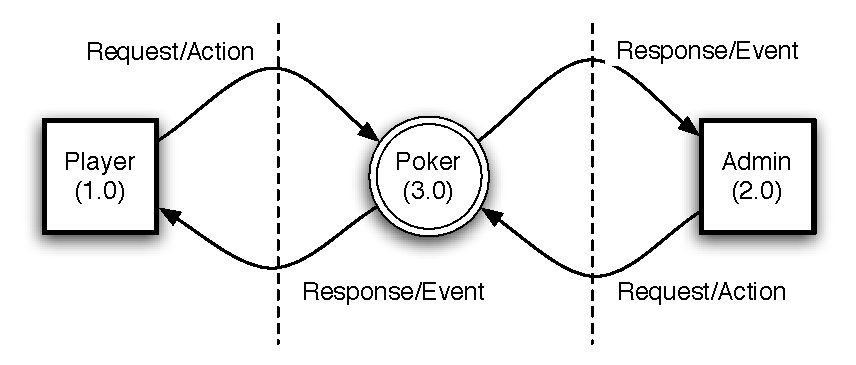
\includegraphics{context_diagram}
  \end{center}
  \caption{Context Level DFD}\label{fig:context}
\end{figure}

\begin{figure}
  \begin{center}
    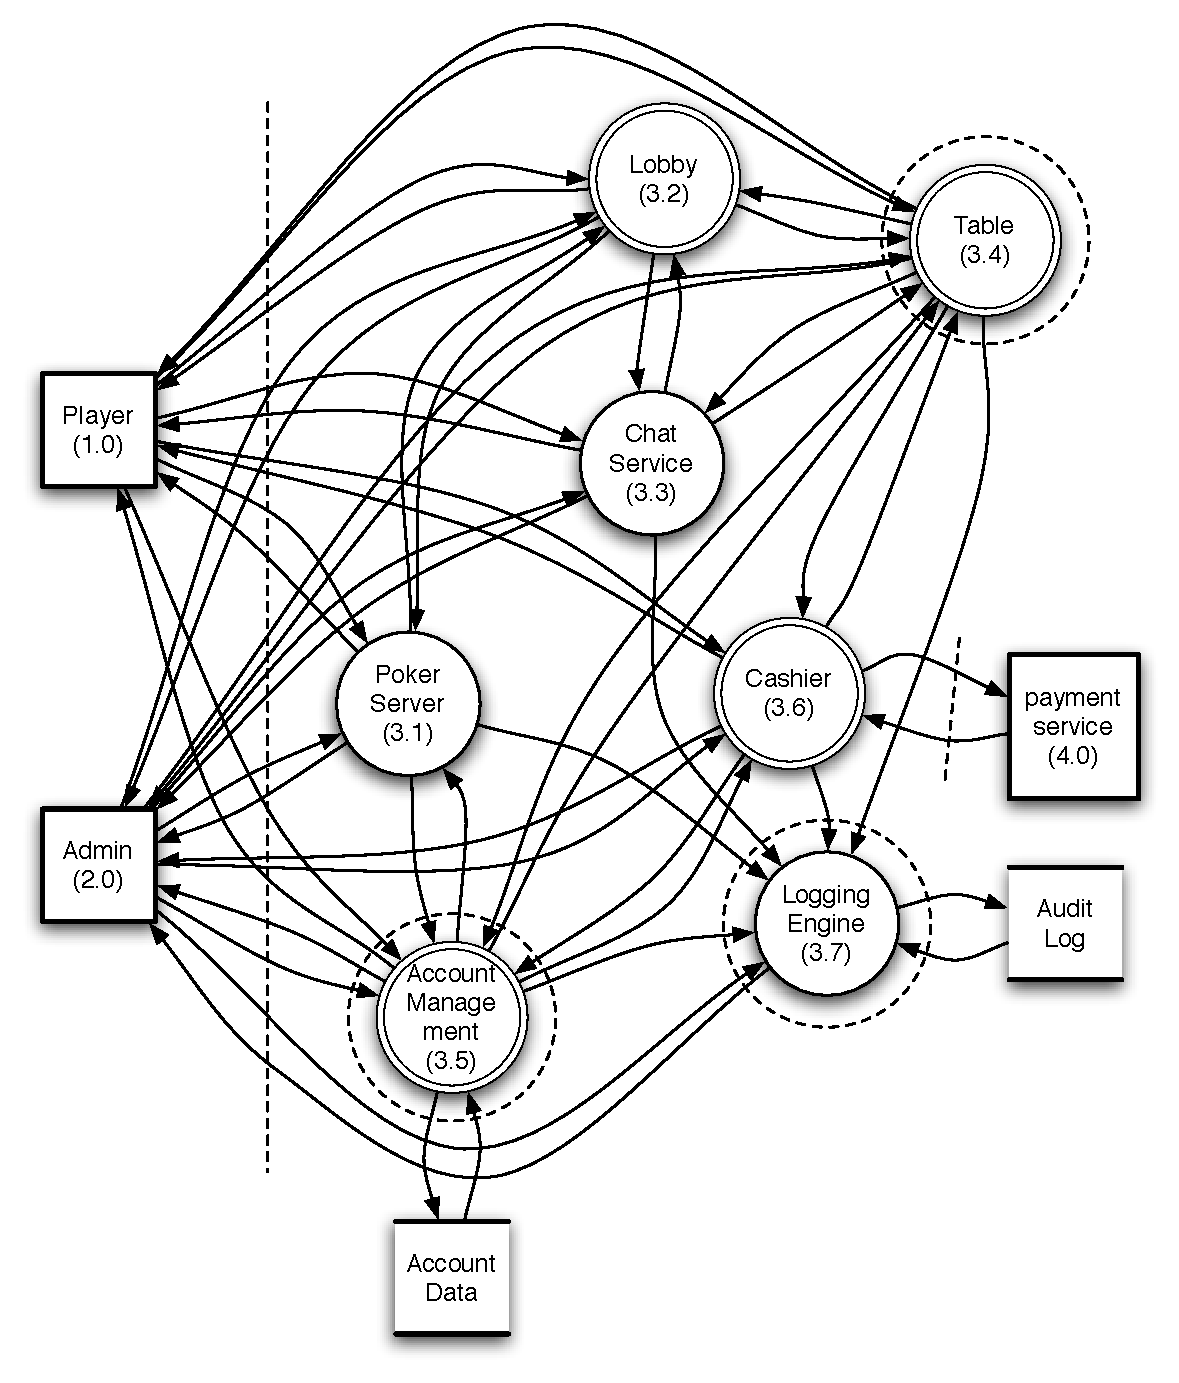
\includegraphics[scale=0.8]{dfd_level_0}
  \end{center}
  \caption{DFD Level 0}\label{fig:level_0}
\end{figure}

\begin{figure}
  \begin{center}
    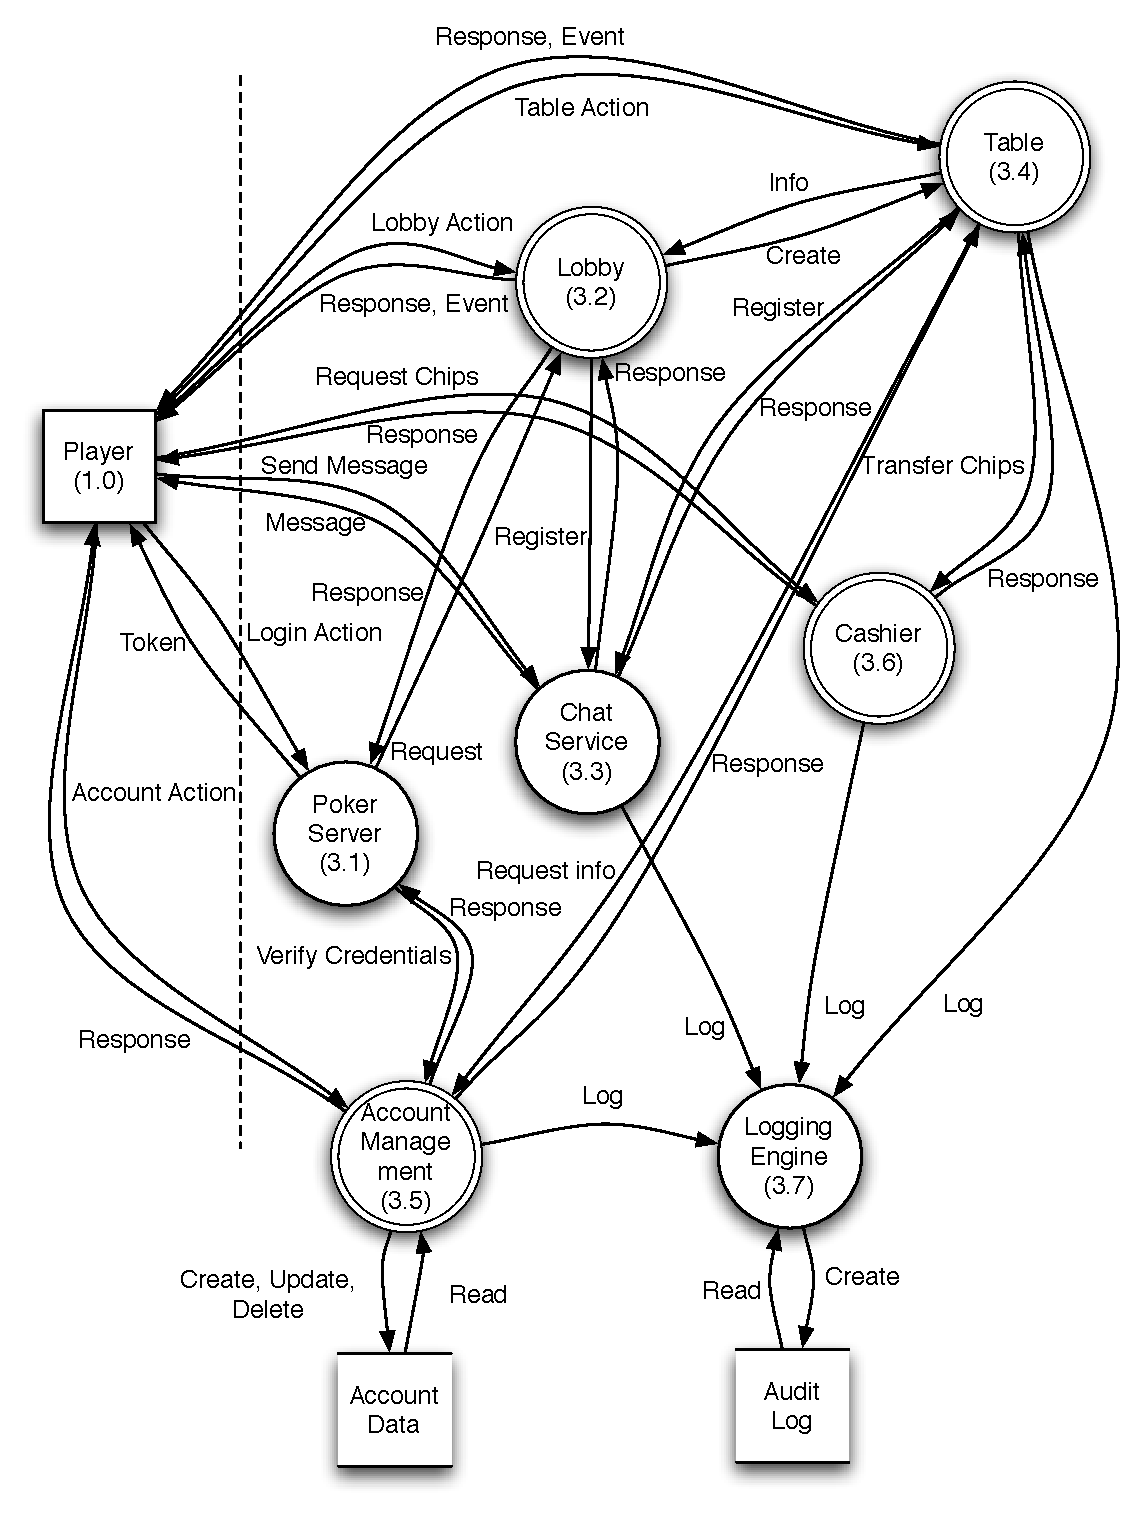
\includegraphics[scale=0.7]{dfd_level_0_player}
  \end{center}
  \caption{DFD Level 0 - only player}\label{fig:level_0_player}
\end{figure}

\section{Rationale}
\subsection{Assumptions}
\begin{itemize}
\item Not protecting application from administrators with debuggers.
\end{itemize}

\section{Misuse Cases}
\subsection{Template}
\textbf{Primary mis-actor:}
\begin{itemize}
\item 
\end{itemize}
\textbf{Basic path:}
\begin{itemize}
\item 
\end{itemize}
\textbf{Alternative paths:}
\begin{itemize}
\item 
\end{itemize}
\textbf{Capture points:}
\begin{itemize}
\item \textbf{Prevention:}
\begin{itemize}
\item 
\end{itemize}
\item \textbf{Detection:}
\begin{itemize}
\item 
\end{itemize}
\end{itemize}

\subsection{Player}
\subsubsection{Spoofing a Player}
\textbf{Primary mis-actor:}
\begin{itemize}
\item Crook
\end{itemize}
\textbf{Basic path:}
\begin{itemize}
\item The mis-actor obtains the credentials of a legitimate player or finds a way to fake credentials.
\item The mis-actor authenticates with the poker server.
\item The mis-actor can take actions on behalf of a legitimate player.
\end{itemize}
\textbf{Alternative paths:}
\begin{itemize}
\item The mis-actor bypasses the authentication system by exploiting a weakness.
\end{itemize}
\textbf{Capture points:}
\begin{itemize}
\item \textbf{Prevention:}
\begin{itemize}
\item Make sure credentials are well protected on the server side.
\item Transmit credentials over the wire securely.
\item Test credentials for uniqueness and complexity.
\end{itemize}
\item \textbf{Detection:}
\begin{itemize}
\item Validate input.
\end{itemize}
\end{itemize}

\subsubsection{Repudiation of a Player}
\textbf{Primary mis-actor:}
\begin{itemize}
\item Crook
\end{itemize}
\textbf{Basic path:}
\begin{itemize}
\item The mis-actor prepares the process that can spoof a poker server.
\item The mis-actor deploys its process on the online casino servers (performed by a skilled insider).
\item The mis-actor can cheat and steal sensitive data from the users.
\end{itemize}
\textbf{Alternative paths:}
\begin{itemize}
\item The mis-actor deploys its process on an external server (performed by a skilled outsider).
\end{itemize}
\textbf{Capture points:}
\begin{itemize}
\item \textbf{Prevention:}
\begin{itemize}
\item Only administrators of the online casino can place code on the online poker servers.
\item Only the code that is running on trusted locations can be used as part of the system.
\item Poker servers are authenticated.
\item Messages coming out of the repository are signed.
\end{itemize}
\end{itemize}

\subsection{Poker Server}
\subsubsection{Spoofing the poker server}
\textbf{Primary mis-actor:}
\begin{itemize}
\item Crook
\end{itemize}
\textbf{Basic path:}
\begin{itemize}
\item The mis-actor prepares the process that can spoof a poker server.
\item The mis-actor deploys its process on the online casino servers (performed by a skilled insider).
\item The mis-actor can cheat and steal sensitive data from the users.
\end{itemize}
\textbf{Alternative paths:}
\begin{itemize}
\item The mis-actor deploys its process on an external server (performed by a skilled outsider).
\end{itemize}
\textbf{Capture points:}
\begin{itemize}
\item \textbf{Prevention:}
\begin{itemize}
\item Only administrators of the online casino can place code on the online poker servers.
\item Only the code that is running on trusted locations can be used as part of the system.
\item Poker servers are authenticated.
\item Messages coming out of the poker server are signed.
\end{itemize}
\end{itemize}

\subsubsection{Tampering with the poker server}
\textbf{Primary mis-actor:}
\begin{itemize}
\item Crook
\end{itemize}
\textbf{Basic path:}
\begin{itemize}
\item The mis-actor sends invalid input to the poker server.
\item The message corrupts the state of the poker server. 
\item While the poker server is in the corrupted state, the mis-actor controls the behavior of that poker server.
\item The mis-actor can cheat and steal sensitive data from the users.
\end{itemize}
\textbf{Alternative paths:}
\begin{itemize}
\item The mis-actor provides false credentials (spoofing an administrator) and modifies the poker server.
\end{itemize}
\textbf{Capture points:}
\begin{itemize}
\item \textbf{Prevention:}
\begin{itemize}
\item All input is validated.
\item Spoofing an administrator should be impossible.
\end{itemize}
\end{itemize}

\subsubsection{Repudiation of an action at the poker server}
\textbf{Primary mis-actor:}
\begin{itemize}
\item Crook
\end{itemize}
\textbf{Basic path:}
\begin{itemize}
\item The mis-actor performs an action at the poker server.
\item The mis-actor denies he performed the action.
\end{itemize}
\textbf{Alternative paths:}
\begin{itemize}
\item 
\end{itemize}
\textbf{Capture points:}
\begin{itemize}
\item \textbf{Prevention:}
\begin{itemize}
\item 
\end{itemize}
\item \textbf{Detection:}
\begin{itemize}
\item 
\end{itemize}
\end{itemize}
\subsubsection{Information disclosure at the poker server}
\textbf{Primary mis-actor:}
\begin{itemize}
\item Crook
\end{itemize}
\textbf{Basic path:}
\begin{itemize}
\item The mis-actor spoofs an other actor with access to private information (e.g. user names, passwords, ...).
\item The mis-actor uses the private information.
\end{itemize}
\textbf{Alternative paths:}
\begin{itemize}
\item Elevation of privilege of the mis-actor leads to information disclosure.
\item The mis-actor sends invalid input to the poker server.
\item The mis-actor has access to the memory and can alter its state (e.g. debugging mode).
\end{itemize}
\textbf{Capture points:}
\begin{itemize}
\item \textbf{Prevention:}
\begin{itemize}
\item 
\end{itemize}
\item \textbf{Detection:}
\begin{itemize}
\item 
\end{itemize}
\end{itemize}

\subsubsection{DoS against the poker server}
\textbf{Primary mis-actor:}
\begin{itemize}
\item Crook
\end{itemize}
\textbf{Basic path:}
\begin{itemize}
\item The mis-actor sends invalid input to the poker server. 
\item The poker server crashes.
\item The poker server becomes unavailable.
\end{itemize}
\textbf{Alternative paths:}
\begin{itemize}
\item The mis-actor crashes the poker server by tampering with the poker server.
\item The mis-actor consumes application-specific resources (e.g. send more login requests per second than the poker server can handle).
\item The mis-actor consumes fundamental resources.
\end{itemize}
\textbf{Capture points:}
\begin{itemize}
\item \textbf{Prevention:}
\begin{itemize}
\item All input is validated.
\item The poker server is load-balanced.
\end{itemize}
\item \textbf{Detection:}
\begin{itemize}
\item Access to the poker server is securely logged.
\end{itemize}
\end{itemize}

\subsubsection{Elevation of privilege at the poker server}
textbf{Primary mis-actor:}
\begin{itemize}
\item Crook
\end{itemize}
\textbf{Basic path:}
\begin{itemize}
\item The mis-actor logs in.
\item He activates the role (administrator) with higher privileges.
\item The mis-actor gains higher privileges. 
\item The mis-actor misuses the higher privileges.
\end{itemize}
\textbf{Alternative paths:}
\begin{itemize}
\item The mis-actor spoofs the identity of an other actor (administrator) with higher privileges.
\item The mis-actor tampers with the poker server to gain more privileges. 
\item The mis-actor sends invalid input to the poker server. 
\item The mis-actor has access to the memory and can alter its state (e.g. debugging mode).
\end{itemize}
\textbf{Capture points:}
\begin{itemize}
\item \textbf{Prevention:}
\begin{itemize}
\item Authentication and authorisation system that verifies credentials.
\item Spoofing user and tampering with poker server prevention.
\end{itemize}
\item \textbf{Detection:}
\begin{itemize}
\item Access to the poker server is securely logged. The log can be compared with the security policy to verify if an actor is allowed to do the action.
\end{itemize}
\end{itemize}

\subsection{Lobby}
\subsection{Table}
\subsubsection{Spoofing a table}
\textbf{Primary mis-actor:}
\begin{itemize}
\item 
\end{itemize}
\textbf{Basic path:}
\begin{itemize}
\item 
\end{itemize}
\textbf{Alternative paths:}
\begin{itemize}
\item 
\end{itemize}
\textbf{Capture points:}
\begin{itemize}
\item \textbf{Prevention:}
\begin{itemize}
\item 
\end{itemize}
\item \textbf{Detection:}
\begin{itemize}
\item 
\end{itemize}
\end{itemize}
\subsubsection{Tampering with a table}
\textbf{Primary mis-actor:}
\begin{itemize}
\item 
\end{itemize}
\textbf{Basic path:}
\begin{itemize}
\item 
\end{itemize}
\textbf{Alternative paths:}
\begin{itemize}
\item 
\end{itemize}
\textbf{Capture points:}
\begin{itemize}
\item \textbf{Prevention:}
\begin{itemize}
\item 
\end{itemize}
\item \textbf{Detection:}
\begin{itemize}
\item 
\end{itemize}
\end{itemize}
\subsubsection{Repudiation of a table}
\textbf{Primary mis-actor:}
\begin{itemize}
\item 
\end{itemize}
\textbf{Basic path:}
\begin{itemize}
\item 
\end{itemize}
\textbf{Alternative paths:}
\begin{itemize}
\item 
\end{itemize}
\textbf{Capture points:}
\begin{itemize}
\item \textbf{Prevention:}
\begin{itemize}
\item 
\end{itemize}
\item \textbf{Detection:}
\begin{itemize}
\item 
\end{itemize}
\end{itemize}
\subsubsection{Information disclosure of a table}
\textbf{Primary mis-actor:}
\begin{itemize}
\item 
\end{itemize}
\textbf{Basic path:}
\begin{itemize}
\item 
\end{itemize}
\textbf{Alternative paths:}
\begin{itemize}
\item 
\end{itemize}
\textbf{Capture points:}
\begin{itemize}
\item \textbf{Prevention:}
\begin{itemize}
\item 
\end{itemize}
\item \textbf{Detection:}
\begin{itemize}
\item 
\end{itemize}
\end{itemize}
\subsubsection{DoS against a table}
\textbf{Primary mis-actor:}
\begin{itemize}
\item 
\end{itemize}
\textbf{Basic path:}
\begin{itemize}
\item 
\end{itemize}
\textbf{Alternative paths:}
\begin{itemize}
\item 
\end{itemize}
\textbf{Capture points:}
\begin{itemize}
\item \textbf{Prevention:}
\begin{itemize}
\item 
\end{itemize}
\item \textbf{Detection:}
\begin{itemize}
\item 
\end{itemize}
\end{itemize}
\subsubsection{Elevation of Privilege}
\subsection{Chat Service}
\subsection{Cashier}
\subsection{Account Management}
\subsubsection{Spoofing the account management system}
\textbf{Primary mis-actor:}
\begin{itemize}
\item 
\end{itemize}
\textbf{Basic path:}
\begin{itemize}
\item 
\end{itemize}
\textbf{Alternative paths:}
\begin{itemize}
\item 
\end{itemize}
\textbf{Capture points:}
\begin{itemize}
\item \textbf{Prevention:}
\begin{itemize}
\item 
\end{itemize}
\item \textbf{Detection:}
\begin{itemize}
\item 
\end{itemize}
\end{itemize}
\subsubsection{Tampering with the account management system}
\textbf{Primary mis-actor:}
\begin{itemize}
\item 
\end{itemize}
\textbf{Basic path:}
\begin{itemize}
\item 
\end{itemize}
\textbf{Alternative paths:}
\begin{itemize}
\item 
\end{itemize}
\textbf{Capture points:}
\begin{itemize}
\item \textbf{Prevention:}
\begin{itemize}
\item 
\end{itemize}
\item \textbf{Detection:}
\begin{itemize}
\item 
\end{itemize}
\end{itemize}
\subsubsection{Repudiation of using the account management system}
\textbf{Primary mis-actor:}
\begin{itemize}
\item 
\end{itemize}
\textbf{Basic path:}
\begin{itemize}
\item 
\end{itemize}
\textbf{Alternative paths:}
\begin{itemize}
\item 
\end{itemize}
\textbf{Capture points:}
\begin{itemize}
\item \textbf{Prevention:}
\begin{itemize}
\item 
\end{itemize}
\item \textbf{Detection:}
\begin{itemize}
\item 
\end{itemize}
\end{itemize}
\subsubsection{Information disclosure of the account management system}
\textbf{Primary mis-actor:}
\begin{itemize}
\item 
\end{itemize}
\textbf{Basic path:}
\begin{itemize}
\item 
\end{itemize}
\textbf{Alternative paths:}
\begin{itemize}
\item 
\end{itemize}
\textbf{Capture points:}
\begin{itemize}
\item \textbf{Prevention:}
\begin{itemize}
\item 
\end{itemize}
\item \textbf{Detection:}
\begin{itemize}
\item 
\end{itemize}
\end{itemize}
\subsubsection{DoS against the account management system}
\textbf{Primary mis-actor:}
\begin{itemize}
\item 
\end{itemize}
\textbf{Basic path:}
\begin{itemize}
\item 
\end{itemize}
\textbf{Alternative paths:}
\begin{itemize}
\item 
\end{itemize}
\textbf{Capture points:}
\begin{itemize}
\item \textbf{Prevention:}
\begin{itemize}
\item 
\end{itemize}
\item \textbf{Detection:}
\begin{itemize}
\item 
\end{itemize}
\end{itemize}
\subsubsection{Elevation of Privilege}
\textbf{Primary mis-actor:}
\begin{itemize}
\item 
\end{itemize}
\textbf{Basic path:}
\begin{itemize}
\item 
\end{itemize}
\textbf{Alternative paths:}
\begin{itemize}
\item 
\end{itemize}
\textbf{Capture points:}
\begin{itemize}
\item \textbf{Prevention:}
\begin{itemize}
\item 
\end{itemize}
\item \textbf{Detection:}
\begin{itemize}
\item 
\end{itemize}
\end{itemize}
\subsection{Account Data}
\subsubsection{Tampering with account data}
\textbf{Primary mis-actor:}
\begin{itemize}
\item Crook
\end{itemize}
\textbf{Basic path:}
\begin{itemize}
\item The mis-actor gains access to the data store
\item The mis-actor puts date directly in the data store
\end{itemize}
\textbf{Alternative paths:}
\begin{itemize}
\item The mis-actor removes data directly from the data store
\item There may be overcapacity failures: the mis-actor floods the data store by placing large 
amounts of data into the data store. As a consequence data in the beginning of the store might be overwritten
, data written to the store might be discarded or the data store might crash, depending on the implementation of
the data store.
\end{itemize}
\textbf{Capture points:}
\begin{itemize}
\item \textbf{Prevention:}
\begin{itemize}
\item placing and removing of data in the data store is securely logged
\item data store is protected by the internal policies
\item extra-monitor access is impossible (behind a reliable firewall)
\item overcapacity failures are handled accordingly
\item only private or local networks are used for communication between the account management process 
and the account data store.
\end{itemize}
\item \textbf{Detection:}
\begin{itemize}
\item logs can be searched for adding of removing falsified data
\end{itemize}
\end{itemize}

\subsubsection{Information disclosure of account data}
\textbf{Primary mis-actor:}
\begin{itemize}
\item 
\end{itemize}
\textbf{Basic path:}
\begin{itemize}
\item 
\end{itemize}
\textbf{Alternative paths:}
\begin{itemize}
\item 
\end{itemize}
\textbf{Capture points:}
\begin{itemize}
\item \textbf{Prevention:}
\begin{itemize}
\item 
\end{itemize}
\item \textbf{Detection:}
\begin{itemize}
\item 
\end{itemize}
\end{itemize}

\subsubsection{DoS against account data}
\textbf{Primary mis-actor:}
\begin{itemize}
\item 
\end{itemize}
\textbf{Basic path:}
\begin{itemize}
\item 
\end{itemize}
\textbf{Alternative paths:}
\begin{itemize}
\item 
\end{itemize}
\textbf{Capture points:}
\begin{itemize}
\item \textbf{Prevention:}
\begin{itemize}
\item 
\end{itemize}
\item \textbf{Detection:}
\begin{itemize}
\item 
\end{itemize}
\end{itemize}
\textbf{Primary mis-actor:}
\begin{itemize}
\item 
\end{itemize}
\textbf{Basic path:}
\begin{itemize}
\item 
\end{itemize}
\textbf{Alternative paths:}
\begin{itemize}
\item 
\end{itemize}
\textbf{Capture points:}
\begin{itemize}
\item \textbf{Prevention:}
\begin{itemize}
\item 
\end{itemize}
\item \textbf{Detection:}
\begin{itemize}
\item 
\end{itemize}
\end{itemize}
\textbf{Primary mis-actor:}
\begin{itemize}
\item 
\end{itemize}
\textbf{Basic path:}
\begin{itemize}
\item 
\end{itemize}
\textbf{Alternative paths:}
\begin{itemize}
\item 
\end{itemize}
\textbf{Capture points:}
\begin{itemize}
\item \textbf{Prevention:}
\begin{itemize}
\item 
\end{itemize}
\item \textbf{Detection:}
\begin{itemize}
\item 
\end{itemize}
\end{itemize}
\subsection{Logging Engine}
\subsubsection{Spoofing the logging engine}
\textbf{Primary mis-actor:}
\begin{itemize}
\item 
\end{itemize}
\textbf{Basic path:}
\begin{itemize}
\item 
\end{itemize}
\textbf{Alternative paths:}
\begin{itemize}
\item 
\end{itemize}
\textbf{Capture points:}
\begin{itemize}
\item \textbf{Prevention:}
\begin{itemize}
\item 
\end{itemize}
\item \textbf{Detection:}
\begin{itemize}
\item 
\end{itemize}
\end{itemize}
\subsubsection{Tampering with the logging engine}
\textbf{Primary mis-actor:}
\begin{itemize}
\item 
\end{itemize}
\textbf{Basic path:}
\begin{itemize}
\item 
\end{itemize}
\textbf{Alternative paths:}
\begin{itemize}
\item 
\end{itemize}
\textbf{Capture points:}
\begin{itemize}
\item \textbf{Prevention:}
\begin{itemize}
\item 
\end{itemize}
\item \textbf{Detection:}
\begin{itemize}
\item 
\end{itemize}
\end{itemize}
\subsubsection{Repudiation of using the logging engine}
\textbf{Primary mis-actor:}
\begin{itemize}
\item 
\end{itemize}
\textbf{Basic path:}
\begin{itemize}
\item 
\end{itemize}
\textbf{Alternative paths:}
\begin{itemize}
\item 
\end{itemize}
\textbf{Capture points:}
\begin{itemize}
\item \textbf{Prevention:}
\begin{itemize}
\item 
\end{itemize}
\item \textbf{Detection:}
\begin{itemize}
\item 
\end{itemize}
\end{itemize}
\subsubsection{Information disclosure of the logging engine}
\textbf{Primary mis-actor:}
\begin{itemize}
\item 
\end{itemize}
\textbf{Basic path:}
\begin{itemize}
\item 
\end{itemize}
\textbf{Alternative paths:}
\begin{itemize}
\item 
\end{itemize}
\textbf{Capture points:}
\begin{itemize}
\item \textbf{Prevention:}
\begin{itemize}
\item 
\end{itemize}
\item \textbf{Detection:}
\begin{itemize}
\item 
\end{itemize}
\end{itemize}
\subsubsection{DoS against the logging engine}
\textbf{Primary mis-actor:}
\begin{itemize}
\item 
\end{itemize}
\textbf{Basic path:}
\begin{itemize}
\item 
\end{itemize}
\textbf{Alternative paths:}
\begin{itemize}
\item 
\end{itemize}
\textbf{Capture points:}
\begin{itemize}
\item \textbf{Prevention:}
\begin{itemize}
\item 
\end{itemize}
\item \textbf{Detection:}
\begin{itemize}
\item 
\end{itemize}
\end{itemize}
\subsubsection{Elevation of Privilege}
\textbf{Primary mis-actor:}
\begin{itemize}
\item 
\end{itemize}
\textbf{Basic path:}
\begin{itemize}
\item 
\end{itemize}
\textbf{Alternative paths:}
\begin{itemize}
\item 
\end{itemize}
\textbf{Capture points:}
\begin{itemize}
\item \textbf{Prevention:}
\begin{itemize}
\item 
\end{itemize}
\item \textbf{Detection:}
\begin{itemize}
\item 
\end{itemize}
\end{itemize}
\subsection{Audit Log}
\subsubsection{Tampering with the audit log}
\textbf{Primary mis-actor:}
\begin{itemize}
\item 
\end{itemize}
\textbf{Basic path:}
\begin{itemize}
\item 
\end{itemize}
\textbf{Alternative paths:}
\begin{itemize}
\item 
\end{itemize}
\textbf{Capture points:}
\begin{itemize}
\item \textbf{Prevention:}
\begin{itemize}
\item 
\end{itemize}
\item \textbf{Detection:}
\begin{itemize}
\item 
\end{itemize}
\end{itemize}

\subsubsection{Information disclosure of the audit log}
\textbf{Primary mis-actor:}
\begin{itemize}
\item 
\end{itemize}
\textbf{Basic path:}
\begin{itemize}
\item 
\end{itemize}
\textbf{Alternative paths:}
\begin{itemize}
\item 
\end{itemize}
\textbf{Capture points:}
\begin{itemize}
\item \textbf{Prevention:}
\begin{itemize}
\item 
\end{itemize}
\item \textbf{Detection:}
\begin{itemize}
\item 
\end{itemize}
\end{itemize}

\subsubsection{DoS against account data}
\end{document} 